% Section V: Results
\section{Results}
\label{sec:resultados}

Unless stated otherwise, results are on CIFAR-10 with 400 epochs. Accuracies are given as mean $\pm$ standard deviation across seeds, and differences ($\Delta$) are paired by seed against the stated reference. Variant names follow Table~\ref{tab:variantes}: \var{dot} is the base model; the suffix \var{\_wide} marks an equal-capacity control with a wider MLP; \var{\_local} and \var{\_local\_k5} add the $3\times3$ and $5\times5$ local terms; \var{ham\_concat} is \var{dot} with the \emph{pooling} branch fused by concatenation; and \var{ham\_concat\_local\_k5} is the triad, whose equal-capacity control is \var{dot\_wide\_local\_k5}.

\subsection{Performance Metrics}
\label{sec:desempeno}

\subsubsection{Fusing Two Attention Mechanisms Does Not Improve Dot-Product Attention}
\label{sec:res-fusiones}
Table~\ref{tab:fusiones} summarizes the fusions of the first family. None beats \var{dot} significantly after Holm correction. The best, \var{ham\_concat} ($+0.46$ points with 5 seeds), combines \var{dot} with the \emph{pooling} branch, which is not a second similarity function but a global summary. Fusions of two pairwise branches range between $+0.29$ and $-0.55$, and the additive branches alone fall below \var{dot} ($-0.29$ and $-0.61$).

% Translated by scripts/tables_en.py from the Spanish table generated by scripts/ieee_tables.py a partir de los runs; no editar a mano.

\begin{table*}[!t]
\centering
\small
\caption{Fusions of two attention mechanisms on CIFAR-10 (400 epochs, seeds 0--4). $\Delta$: paired difference by seed against \texttt{dot} (80.04 $\pm$ 0.31), with Student's t 95~\% CI; Holm over the 13 comparisons.}
\label{tab:fusiones}
\begin{adjustbox}{max width=\linewidth}
\begin{tabular}{lccccc}
\toprule
Variant & Accuracy (\%) & $\Delta$ [95~\% CI] & $\Delta>0$ & $p$ & $p$ Holm \\
\midrule
\texttt{ham\_concat} & 80.50 $\pm$ 0.65 & $+0.46$ [$-0.36$, $+1.27$] & 4/5 & 0.194 & 1.000 \\
\texttt{ham\_weighted\_learn\_out} & 80.33 $\pm$ 0.61 & $+0.29$ [$-0.21$, $+0.79$] & 4/5 & 0.184 & 1.000 \\
\texttt{ham\_heads} & 80.24 $\pm$ 0.63 & $+0.20$ [$-0.42$, $+0.82$] & 2/5 & 0.415 & 1.000 \\
\texttt{ham\_zscore} & 80.12 $\pm$ 0.48 & $+0.08$ [$-0.42$, $+0.57$] & 3/5 & 0.685 & 1.000 \\
\texttt{ham\_gated} & 79.96 $\pm$ 0.46 & $-0.08$ [$-0.66$, $+0.49$] & 2/5 & 0.707 & 1.000 \\
\texttt{ham\_pairwise} & 79.95 $\pm$ 0.54 & $-0.09$ [$-0.73$, $+0.55$] & 2/5 & 0.721 & 1.000 \\
\texttt{ham\_wout} & 79.81 $\pm$ 0.21 & $-0.23$ [$-0.85$, $+0.39$] & 2/5 & 0.359 & 1.000 \\
\texttt{additive\_free} & 79.75 $\pm$ 0.29 & $-0.29$ [$-0.73$, $+0.14$] & 1/5 & 0.135 & 1.000 \\
\texttt{dot\_wide} & 79.73 $\pm$ 0.63 & $-0.31$ [$-1.18$, $+0.56$] & 2/5 & 0.374 & 1.000 \\
\texttt{ham\_weighted} & 79.66 $\pm$ 0.57 & $-0.38$ [$-1.04$, $+0.28$] & 1/5 & 0.183 & 1.000 \\
\texttt{ham\_weighted\_learn} & 79.53 $\pm$ 0.46 & $-0.51$ [$-1.04$, $+0.02$] & 0/5 & 0.054 & 0.599 \\
\texttt{ham\_sum} & 79.49 $\pm$ 0.32 & $-0.55$ [$-0.99$, $-0.11$] & 0/5 & 0.026 & 0.306 \\
\texttt{additive} & 79.43 $\pm$ 0.33 & $-0.61$ [$-1.07$, $-0.16$] & 0/5 & 0.020 & 0.266 \\
\bottomrule
\end{tabular}
\end{adjustbox}
\end{table*}


With 16 seeds (Table~\ref{tab:principal}), \var{ham\_concat} does beat \var{dot}: $+0.48$ [$+0.19$, $+0.78$], 12 of 16 seeds, Holm $p=0.007$. However, the capacity control \var{dot\_wide}, with the same parameters in the MLP, gains $+0.33$, and the difference between the two is $+0.15$ [$-0.31$, $+0.61$], with 8 of 16 seeds in favor (Table~\ref{tab:contrastes}). The accuracy gain of the original HAM formulation cannot be distinguished from that of adding parameters.

Outside CIFAR-10 with data augmentation the pattern holds (Table~\ref{tab:otros}). Without data augmentation, the \emph{pooling} branch alone obtains $+0.71$ (not significant) and the score sum falls below \var{dot} ($-1.07$, Holm $p=0.043$). On Food-101, \var{ham\_concat} gives $+0.40$ and the additive branch alone $-0.60$, both non-significant. On PlantVillage (Section~\ref{sec:res-pv}) the additive branches do improve on \var{dot}, but no fusion beats the additive branch alone.

% Translated by scripts/tables_en.py from the Spanish table generated by scripts/ieee_tables.py a partir de los runs; no editar a mano.

\begin{table*}[!t]
\centering
\small
\caption{Fusions in other regimes (seeds 0--4). CIFAR-10 without data augmentation (400 epochs) and Food-101 ($192\times192$, patches of 8, 50 epochs, batch 128). Holm within each block.}
\label{tab:otros}
\begin{adjustbox}{max width=\linewidth}
\begin{tabular}{llcccc}
\toprule
Regime & Variant & Accuracy (\%) & $\Delta$ [95~\% CI] & $\Delta>0$ & $p$ Holm \\
\midrule
CIFAR-10, no augmentation & \texttt{dot} & 76.33 $\pm$ 0.36 & --- & --- & --- \\
 & \texttt{additive} & 77.04 $\pm$ 0.52 & $+0.71$ [$-0.25$, $+1.68$] & 4/5 & 0.300 \\
 & \texttt{ham\_concat} & 76.52 $\pm$ 0.50 & $+0.19$ [$-0.50$, $+0.89$] & 3/5 & 0.481 \\
 & \texttt{ham\_weighted} & 75.67 $\pm$ 0.33 & $-0.66$ [$-1.51$, $+0.20$] & 1/5 & 0.300 \\
 & \texttt{ham\_sum} & 75.26 $\pm$ 0.37 & $-1.07$ [$-1.73$, $-0.41$] & 0/5 & 0.043 \\
\midrule
Food-101 & \texttt{dot} & 44.48 $\pm$ 0.63 & --- & --- & --- \\
 & \texttt{additive} & 43.89 $\pm$ 0.57 & $-0.60$ [$-1.36$, $+0.17$] & 1/5 & 0.194 \\
 & \texttt{ham\_concat} & 44.88 $\pm$ 0.34 & $+0.40$ [$-0.23$, $+1.02$] & 3/5 & 0.194 \\
\bottomrule
\end{tabular}
\end{adjustbox}
\end{table*}


\subsubsection{A Local Term in the Output of Each Head Gives the Largest Gain}
\label{sec:res-principal}
Table~\ref{tab:principal} gathers the variants of the main comparison with 16 seeds. Adding a $3\times3$ depthwise convolution over the values of each head (\var{dot\_local}) raises accuracy from 79.85 to 84.38~\%: $+4.52$ [$+3.97$, $+5.07$], 16 of 16 seeds. The term adds 1,920 parameters (1.6~\%) and 7~\% to the epoch time. Against the capacity control \var{dot\_wide}, which has 7,780 more parameters, the difference is $+4.19$ [$+3.67$, $+4.71$]: the gain is not a capacity effect.

Widening the neighborhood to $5\times5$ (\var{dot\_local\_k5}) adds $+1.12$ [$+0.61$, $+1.63$] over $3\times3$ (15 of 16 seeds, Holm $p=0.002$), for a total of $+5.64$ over \var{dot} at the same cost per epoch. The triad of inductive biases, \var{ham\_concat\_local\_k5}~\eqref{eq:final}, reaches 86.16 $\pm$ 0.86~\%, the highest accuracy in the study: $+6.31$ [$+5.76$, $+6.86$] over \var{dot}. Its advantage over \var{dot\_local\_k5} is $+0.67$ [$+0.07$, $+1.27$] (13 of 16 seeds; $p=0.032$, Wilcoxon $p=0.021$), which stops being significant after correcting for the seven planned contrasts (Holm $p=0.158$). Against its equal-capacity control, \var{dot\_wide\_local\_k5} (the $5\times5$ local term on the wider MLP; 85.67~\%, 16 seeds), the difference shrinks to $+0.49$ [$-0.24$, $+1.23$] (10 of 16 seeds, Holm $p=0.513$; Table~\ref{tab:contrastes}). With a standard deviation of the paired differences of 1.4 points, detecting an effect of that size required on the order of 60 seeds, so 32 more seeds of both variants were run (16 to 47) with a single contrast declared before running them: the accuracy of the triad minus that of its control, with a paired $t$-test. With the 48 seeds the advantage is $+0.61$ [$+0.17$, $+1.06$] (31 of 48 seeds, $p=0.008$; Wilcoxon $p=0.008$), with means of 86.17 $\pm$ 0.88 and 85.55 $\pm$ 1.05~\%. On the 32 new seeds, which played no part in the decision to extend the experiment, it is $+0.67$ [$+0.09$, $+1.26$] ($p=0.025$; Table~\ref{tab:evidencia}). The triad costs 1.78 times the epoch time of \var{dot} (1.62 times that of its control). Macro F1 follows accuracy in all variants (Table~\ref{tab:calibracion}).

% Translated by scripts/tables_en.py from the Spanish table generated by scripts/ieee_tables.py a partir de los runs; no editar a mano.

\begin{table*}[!t]
\centering
\footnotesize
\caption{Main results on CIFAR-10 with 16 seeds (0--15), 400 epochs. $\Delta$: paired difference against \texttt{dot}; $p$ with Holm over 6 comparisons. Epoch $\geq$79: first epoch with validation accuracy $\geq$79~\%, mean over the seeds that reach it.}
\label{tab:principal}
\begin{adjustbox}{max width=\linewidth}
\begin{tabular}{lrcccccr}
\toprule
Variant & Params. & Accuracy (\%) & $\Delta$ [95~\% CI] & $\Delta>0$ & $p$ Holm & Epoch $\geq$79 & s/epoch \\
\midrule
\texttt{dot} & 119\,290 & 79.85 $\pm$ 0.54 & --- & --- & --- & 234 (15/16) & 1.38 \\
\texttt{dot\_wide} & 128\,990 & 80.19 $\pm$ 0.56 & $+0.33$ [$-0.15$, $+0.81$] & 11/16 & 0.160 & 213 (15/16) & 1.41 \\
\texttt{ham\_concat} & 128\,906 & 80.34 $\pm$ 0.43 & $+0.48$ [$+0.19$, $+0.78$] & 12/16 & 0.007 & 204 & 2.32 \\
\texttt{dot\_local} & 121\,210 & 84.38 $\pm$ 0.84 & $+4.52$ [$+3.97$, $+5.07$] & 16/16 & $<0.001$ & 75 & 1.48 \\
\texttt{dot\_local\_k5} & 124\,282 & 85.49 $\pm$ 0.90 & $+5.64$ [$+5.07$, $+6.21$] & 16/16 & $<0.001$ & 59 & 1.49 \\
\texttt{dot\_wide\_local\_k5} & 133\,982 & 85.67 $\pm$ 1.02 & $+5.81$ [$+5.23$, $+6.40$] & 16/16 & $<0.001$ & 57 & 1.52 \\
\texttt{ham\_concat\_local\_k5} & 133\,898 & 86.16 $\pm$ 0.86 & $+6.31$ [$+5.76$, $+6.86$] & 16/16 & $<0.001$ & 55 & 2.46 \\
\bottomrule
\end{tabular}
\end{adjustbox}
\end{table*}

% Translated by scripts/tables_en.py from the Spanish table generated by scripts/ieee_tables.py a partir de los runs; no editar a mano.

\begin{table*}[!t]
\centering
\footnotesize
\caption{Planned contrasts on CIFAR-10 with 16 seeds, paired by seed. $p$: paired t-test; Holm over the 7 contrasts; Wilcoxon signed-rank test.}
\label{tab:contrastes}
\begin{adjustbox}{max width=\linewidth}
\begin{tabular}{>{\raggedright\arraybackslash}l>{\raggedright\arraybackslash}p{3.3cm}ccccc}
\toprule
Contrast & What it measures & $\Delta$ [95~\% CI] & $\Delta>0$ & $p$ & $p$ Holm & $p$ Wilcoxon \\
\midrule
\texttt{ham\_concat} $-$ \texttt{dot\_wide} & global branch without locality, at equal capacity & $+0.15$ [$-0.31$, $+0.61$] & 8/16 & 0.491 & 0.981 & 0.940 \\
\texttt{dot\_local} $-$ \texttt{dot\_wide} & $3\times3$ local term against capacity & $+4.19$ [$+3.67$, $+4.71$] & 16/16 & $<0.001$ & $<0.001$ & $<0.001$ \\
\texttt{dot\_local\_gate} $-$ \texttt{dot\_local} & gate on the local term & $-0.11$ [$-0.50$, $+0.28$] & 9/16 & 0.553 & 0.981 & 0.959 \\
\texttt{dot\_local\_k5} $-$ \texttt{dot\_local} & $5\times5$ against $3\times3$ neighborhood & $+1.12$ [$+0.61$, $+1.63$] & 15/16 & $<0.001$ & 0.002 & 0.002 \\
\texttt{ham\_concat\_local\_k5} $-$ \texttt{dot\_local\_k5} & global branch with $5\times5$ locality & $+0.67$ [$+0.07$, $+1.27$] & 13/16 & 0.032 & 0.158 & 0.021 \\
\texttt{ham\_concat} $-$ \texttt{ham\_dotdot} & global branch without locality, against the fusion projection & $+0.37$ [$+0.01$, $+0.73$] & 11/16 & 0.045 & 0.180 & 0.041 \\
\texttt{ham\_concat\_local\_k5} $-$ \texttt{dot\_wide\_local\_k5} & global branch with $5\times5$ locality, at equal capacity & $+0.49$ [$-0.24$, $+1.23$] & 10/16 & 0.171 & 0.513 & 0.144 \\
\bottomrule
\end{tabular}
\end{adjustbox}
\end{table*}


\subsubsection{Calibration and Robustness}
\label{sec:res-calibracion}
The local term also improves calibration and robustness on CIFAR-10 (Table~\ref{tab:calibracion}). ECE drops from 6.71 (\var{dot}) to 5.26 (\var{dot\_local}) and 5.15~\% (\var{dot\_local\_k5}), and NLL from 0.628 to 0.488 and 0.460. \var{ham\_concat\_local\_k5} has the best calibration (ECE of 4.98~\%, NLL of 0.441), in line with the calibration improvement of \var{ham\_concat} over \var{dot} (6.10 versus 6.71~\%). That improvement is reproduced, with 16 seeds, by a control with two identical \var{dot} branches fused with \var{concat\_linear} (ECE of 6.10~\%), but not by \var{dot\_wide} (6.70~\%): it comes from the per-head projection of the fusion, not from the \emph{pooling} branch or the number of parameters. With the local term, the triad is also better calibrated than its equal-capacity control: with 48 seeds, ECE $-0.36$ [$-0.55$, $-0.18$] against \var{dot\_wide\_local\_k5}, 37 of 48 seeds (Holm $p=0.002$; Table~\ref{tab:evidencia}), and NLL $-0.020$ [$-0.033$, $-0.007$] ($p=0.003$). With the first 16 seeds the ECE difference was $-0.29$ ($p=0.031$). With Gaussian noise of $\sigma=0.05$, accuracy goes from 66.5 to 74.8~\% with $5\times5$; with 25~\% occlusion, from 61.1 to 68.3~\%. \var{dot\_local\_k1} improves none of these metrics. Unlike on PlantVillage (Section~\ref{sec:res-pv}), on CIFAR-10 the local term does not worsen robustness to occlusion.

% Translated by scripts/tables_en.py from the Spanish table generated by scripts/ieee_tables.py a partir de los runs; no editar a mano.

\begin{table*}[!t]
\centering
\footnotesize
\caption{Calibration and robustness on CIFAR-10 (mean over the available seeds, $n$). ECE with 15 bins, in \%. Robustness: accuracy (\%) on the full test set with Gaussian noise ($\sigma$ on the image in $[0,1]$), Gaussian blur ($\sigma=1$~px) and random occlusion of 25~\% of the patches.}
\label{tab:calibracion}
\begin{adjustbox}{max width=\linewidth}
\begin{tabular}{lcccccccc}
\toprule
Variant & $n$ & ECE & NLL & F1 macro & Noise 0.05 & Noise 0.1 & Blur 1.0 & Occlusion 25~\% \\
\midrule
\texttt{dot} & 16 & 6.71 & 0.628 & 79.71 & 66.5 & 37.5 & 43.5 & 61.1 \\
\texttt{dot\_wide} & 16 & 6.70 & 0.623 & 80.07 & 67.3 & 38.5 & 42.4 & 61.6 \\
\texttt{ham\_concat} & 16 & 6.10 & 0.609 & 80.19 & 67.0 & 38.0 & 43.5 & 61.3 \\
\texttt{dot\_local\_k1} & 5 & 6.72 & 0.622 & 80.01 & 66.3 & 37.5 & 42.4 & 59.6 \\
\texttt{dot\_local} & 16 & 5.26 & 0.488 & 84.28 & 72.4 & 40.2 & 48.6 & 65.7 \\
\texttt{dot\_local\_k5} & 16 & 5.15 & 0.460 & 85.38 & 74.8 & 43.3 & 52.0 & 68.3 \\
\texttt{dot\_local\_k7} & 5 & 5.43 & 0.460 & 85.44 & 73.4 & 41.3 & 52.5 & 70.0 \\
\texttt{dot\_wide\_local\_k5} & 16 & 5.27 & 0.457 & 85.56 & 74.8 & 42.9 & 51.6 & 68.5 \\
\texttt{ham\_concat\_local\_k5} & 16 & 4.98 & 0.441 & 86.06 & 75.2 & 41.8 & 53.2 & 69.8 \\
\bottomrule
\end{tabular}
\end{adjustbox}
\end{table*}


\subsubsection{Two Training Modes: Where the Gain Comes From}
\label{sec:res-modos}
The final accuracies of the variants with a local term are not unimodal (Fig.~\ref{fig:semillas}). Most seeds of \var{dot\_local} fall between 83.6 and 84.6~\%, but 2 of 16 end between 85.9 and 86.6~\%; in \var{dot}, \var{dot\_wide} and \var{ham\_concat} no seed exceeds 81.6~\%. The high mode is not tied to the seed, because it appears in different seeds depending on the variant, and it is not overfitting: those seeds end with a lower training loss, and the gap between training and validation accuracy is 1.3 to 2.2 points in all the variants of Table~\ref{tab:principal}. None of the attention metrics of Section~\ref{sec:res-capas} distinguishes the seeds of one mode from those of the other.

The frequency of the high mode (test accuracy of at least 85.5~\%, a threshold chosen after observing the distribution; Supplementary Section~\ref{sec:sup-umbral} repeats the counts with thresholds from 85.0 to 86.0~\%) grows with the neighborhood: 0 of 5 seeds with $1\times1$, 2 of 16 with $3\times3$, 9 of 16 with $5\times5$ ($p=0.023$, Fisher, against $3\times3$) and 12 of 16 in \var{ham\_concat\_local\_k5} (8 of 16 in its capacity control; with 48 seeds, 31 versus 21, $p=0.065$, Fisher). With other thresholds the direction of both comparisons is the same, but their significance is not (Supplementary Table~\ref{tab:umbral}). Within each mode, the triad and its control perform almost equally in the high mode (86.75 versus 86.68~\%) and the triad somewhat better in the low mode (85.11 versus 84.67~\%): its advantage comes from entering the high mode more often and from raising the low mode, not from a higher ceiling. The larger neighborhood also shifts the low mode (84.55 versus 84.11~\%, $p=0.009$, Mann--Whitney). This phenomenon explains the spread of the paired differences between variants with a local term (standard deviation of $\sim$1.1 points) and why 5-seed estimates, such as the initial $+1.32$ of \var{ham\_concat\_local\_k5} over \var{dot\_local\_k5}, shrank when seeds were added.

\begin{figure*}[!t]
  \centering
  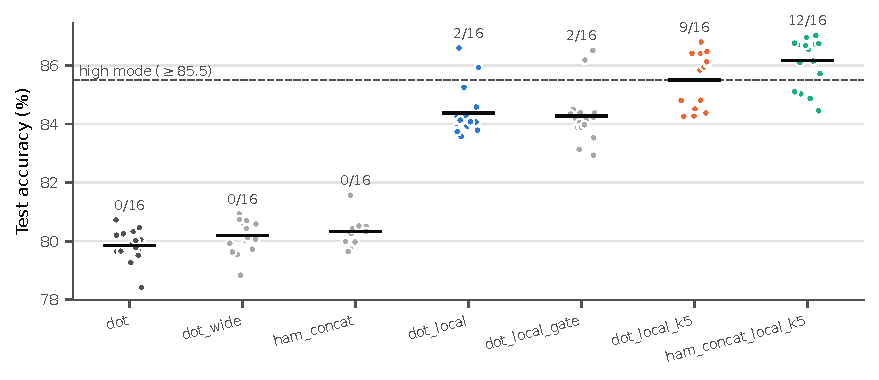
\includegraphics[width=\textwidth]{figuras/semillas.pdf}
  \caption{Test accuracy of each of the 16 seeds. Horizontal bars are the mean, and the numbers are the seeds in the high mode ($\geq 85.5$~\%, dashed line).}
  \label{fig:semillas}
\end{figure*}

\subsubsection{Generalization to PlantVillage}
\label{sec:res-pv}
On PlantVillage (Table~\ref{tab:plantvillage}), where \var{dot} already reaches 97.70~\%, the local term keeps its sign: $+0.46$ with $3\times3$ and $+0.63$ [$+0.38$, $+0.87$] with $5\times5$, 5 of 5 seeds in both cases (Holm $p=0.054$ and $0.019$, over eleven comparisons). On this dataset the additive branches also improve on \var{dot} ($+0.42$ to $+0.64$), but the pairwise branches cost 3.7 to 4.5 times the epoch time of \var{dot}, while the local term costs the same as \var{dot}. \var{dot\_local\_k5} also has the best calibration (ECE of 0.23 versus 0.39~\%) and the highest robustness to noise and blur. Its weak point is occlusion: with 25~\% of the patches erased it obtains 38.7~\%, against 44.9~\% for \var{dot} and 47 to 51~\% for the additive variants.

PlantVillage is also the only dataset on which a second similarity function contributes, and it does so on top of the local term. With the $5\times5$ convolution, the free pairwise additive reaches 98.71~\% ($+1.00$ [$+0.68$, $+1.32$] over \var{dot}) and \var{ham\_sum} 98.74~\% ($+1.04$), close to the sum of the separate effects. Over \var{dot\_local\_k5} they gain $+0.38$ [$+0.13$, $+0.62$] and $+0.42$ [$+0.17$, $+0.66$], in all 5 seeds. The contribution comes from the additive branch and not from the fusion: \var{ham\_sum} remains collapsed onto that branch and performs the same as the additive branch alone ($+0.04$ [$-0.17$, $+0.25$]). The combination costs about four times the epoch time of \var{dot\_local\_k5} and inherits both weaknesses: the occlusion weakness of the local term (38.3~\%) and the noise weakness of the additive branch (34 to 35~\%).

The capacity controls repeat on PlantVillage what was observed on CIFAR-10. Widening the MLP does not help: \var{dot\_wide} gains $+0.06$ over \var{dot} and \var{dot\_wide\_local\_k5} gains $+0.09$ over \var{dot\_local\_k5}. The neighborhood does separate from capacity ($+0.56$ [$+0.12$, $+1.00$] over \var{dot\_wide}, 5 of 5 seeds). The \emph{pooling} branch beats its equal-capacity control in all 5 seeds, without neighborhood ($+0.24$ [$+0.01$, $+0.48$], $p=0.046$) and with it: the triad reaches 98.64~\% and beats \var{dot\_wide\_local\_k5} by $+0.23$ [$-0.05$, $+0.51$] ($p=0.089$). With 5 seeds none of these differences survives correction (Table~\ref{tab:evidencia}), and on this dataset the triad is not better calibrated than its control (ECE $-0.02$). The triad ties with the free additive plus neighborhood ($-0.06$, $p=0.49$), at a third of its epoch time (9.8 versus 29.0~s) and with a lower ECE (0.22 versus 0.29~\%).

% Translated by scripts/tables_en.py from the Spanish table generated by scripts/ieee_tables.py a partir de los runs; no editar a mano.

\begin{table*}[!t]
\centering
\footnotesize
\caption{PlantVillage (38 classes, $64\times64$, 50 epochs, batch 128, seeds 0--4). $\Delta$ paired against \texttt{dot}, Holm over 11 comparisons. ECE in \%. Robustness: accuracy with Gaussian noise $\sigma=0.1$, blur $\sigma=1$~px and occlusion of 25~\% of the patches.}
\label{tab:plantvillage}
\begin{adjustbox}{max width=\linewidth}
\begin{tabular}{lccccrrrrr}
\toprule
Variant & Accuracy (\%) & $\Delta$ [95~\% CI] & $\Delta>0$ & $p$ Holm & s/epoch & ECE & Noise & Blur & Occlusion \\
\midrule
\texttt{dot} & 97.70 $\pm$ 0.25 & --- & --- & --- & 7.7 & 0.39 & 42.2 & 86.8 & 44.9 \\
\texttt{dot\_wide} & 97.77 $\pm$ 0.24 & $+0.06$ [$-0.51$, $+0.64$] & 2/5 & 0.772 & 7.8 & 0.41 & 39.8 & 87.9 & 52.1 \\
\texttt{additive} & 98.12 $\pm$ 0.07 & $+0.42$ [$+0.06$, $+0.78$] & 5/5 & 0.095 & 5.1 & 0.36 & 31.2 & 87.0 & 50.7 \\
\texttt{additive\_free} & 98.22 $\pm$ 0.09 & $+0.52$ [$+0.20$, $+0.84$] & 5/5 & 0.054 & 28.8 & 0.38 & 28.6 & 88.6 & 47.0 \\
\texttt{ham\_concat} & 98.01 $\pm$ 0.14 & $+0.31$ [$-0.11$, $+0.73$] & 5/5 & 0.220 & 9.6 & 0.29 & 40.8 & 87.8 & 49.8 \\
\texttt{ham\_sum} & 98.35 $\pm$ 0.14 & $+0.64$ [$+0.29$, $+1.00$] & 5/5 & 0.043 & 34.8 & 0.31 & 28.2 & 89.2 & 51.5 \\
\texttt{dot\_local} & 98.17 $\pm$ 0.27 & $+0.46$ [$+0.16$, $+0.76$] & 5/5 & 0.054 & 7.8 & 0.30 & 37.9 & 89.9 & 39.7 \\
\texttt{dot\_local\_k5} & 98.33 $\pm$ 0.21 & $+0.63$ [$+0.38$, $+0.87$] & 5/5 & 0.019 & 7.8 & 0.23 & 48.6 & 92.8 & 38.7 \\
\texttt{dot\_wide\_local\_k5} & 98.42 $\pm$ 0.23 & $+0.72$ [$+0.41$, $+1.02$] & 5/5 & 0.022 & 8.0 & 0.24 & 44.4 & 93.4 & 33.6 \\
\texttt{ham\_concat\_local\_k5} & 98.64 $\pm$ 0.13 & $+0.94$ [$+0.50$, $+1.38$] & 5/5 & 0.028 & 9.8 & 0.22 & 44.9 & 94.1 & 35.4 \\
\texttt{additive\_free\_local\_k5} & 98.71 $\pm$ 0.09 & $+1.00$ [$+0.68$, $+1.32$] & 5/5 & 0.011 & 29.0 & 0.29 & 33.7 & 93.7 & 38.3 \\
\texttt{ham\_sum\_local\_k5} & 98.74 $\pm$ 0.11 & $+1.04$ [$+0.68$, $+1.41$] & 5/5 & 0.014 & 32.3 & 0.30 & 35.3 & 93.2 & 38.3 \\
\bottomrule
\end{tabular}
\end{adjustbox}
\end{table*}


\subsubsection{Training Efficiency}
\label{sec:res-eficiencia}
The local term also speeds up learning (Fig.~\ref{fig:curvas}, Table~\ref{tab:eficiencia}). \var{dot} reaches 79~\% validation accuracy at epoch 234 on average (15 of 16 seeds reach it); \var{dot\_local} does so at epoch 75 and \var{dot\_local\_k5} at epoch 59, which amounts to 88~s of GPU time against 323~s, 3.7 times less. Trained for only 100 epochs, \var{dot\_local} reaches 80.01 $\pm$ 0.34~\%, the same as \var{dot} with 400 epochs ($-0.03$ [$-0.50$, $+0.44$], paired by seed). \var{ham\_concat\_local\_k5} needs the fewest epochs (55), but, because of its cost per epoch, not the least GPU time: 136~s, 2.4 times less than \var{dot}, against 3.7 times for \var{dot\_local\_k5}.

\begin{figure}[tbp]
  \centering
  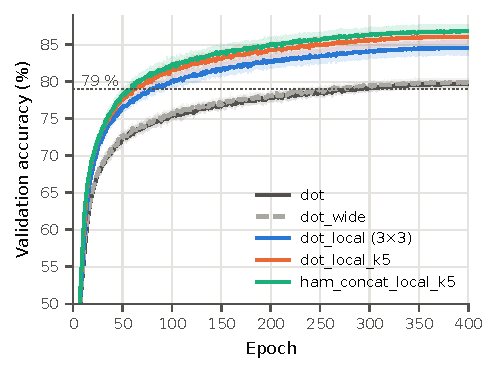
\includegraphics[width=\anchocolumna]{figuras/curvas.pdf}
  \caption{Validation accuracy per epoch on CIFAR-10 (mean $\pm$ standard deviation of 16 seeds). The dotted line marks 79~\%, close to the final value of \var{dot}. The curves of \var{dot} and \var{dot\_wide} overlap.}
  \label{fig:curvas}
\end{figure}

% Translated by scripts/tables_en.py from the Spanish table generated by scripts/ieee_tables.py a partir de los runs; no editar a mano.

\begin{table*}[!t]
\centering
\small
\caption{Training efficiency on CIFAR-10. Epoch and GPU time to reach 79~\% validation accuracy (16 seeds; in parentheses, how many reach it when not all do). Test accuracy when training for 100 epochs (3 warmup epochs; seeds 0--4) and 400 epochs (16 seeds).}
\label{tab:eficiencia}
\begin{adjustbox}{max width=\linewidth}
\begin{tabular}{lcccc}
\toprule
Variant & Epoch $\geq$79 & Time (s) & 100 epochs & 400 epochs \\
\midrule
\texttt{dot} & 234 (15/16) & 323 & 75.85 $\pm$ 0.27 & 79.85 $\pm$ 0.54 \\
\texttt{dot\_wide} & 213 (15/16) & 301 & 76.03 $\pm$ 0.38 & 80.19 $\pm$ 0.56 \\
\texttt{ham\_concat} & 204 & 474 & --- & 80.34 $\pm$ 0.43 \\
\texttt{dot\_local} & 75 & 111 & 80.01 $\pm$ 0.34 & 84.38 $\pm$ 0.84 \\
\texttt{dot\_local\_k5} & 59 & 88 & --- & 85.49 $\pm$ 0.90 \\
\texttt{dot\_wide\_local\_k5} & 57 & 87 & --- & 85.67 $\pm$ 1.02 \\
\texttt{ham\_concat\_local\_k5} & 55 & 136 & --- & 86.16 $\pm$ 0.86 \\
\texttt{dot\_local\_gate} & 70 & 108 & 80.13 $\pm$ 0.28 & 84.27 $\pm$ 0.92 \\
\bottomrule
\end{tabular}
\end{adjustbox}
\end{table*}


\subsubsection{Computational Cost and Inference}
\label{sec:res-costos}
Table~\ref{tab:costos} separates the cost of the variants into hardware-independent quantities and inference measurements. The $5\times5$ local term adds 3.4~\% of MACs (9.27 versus 8.96 million per image) and 4.2~\% of parameters, and it does not change the peak memory of a training step (624~MB) or that of activations (256~KB); its epoch time (1.08 times) is consistent with that arithmetic. The triad, on the other hand, has the same MACs as its capacity control ($+10.3$ versus $+10.4$~\%) and the same memory, but 1.79 times the epoch time against 1.10: the difference comes from the implementation of the \emph{pooling} branch, computed head by head, not from its arithmetic. The opposite happens with the score fusions with pairwise additive attention: \var{ham\_sum} has the MACs of \var{dot}, because the counter does not see the element-wise $\tanh$ over $N\times N\times d$ tensors, but it needs 2.3 times the training memory and 2.5 times the activation memory. Parameter count and MACs are therefore not enough to judge the cost of an attention mechanism.

At inference, with batch 1 and one CPU thread, the models take 0.55 to 2.5~ms per image and weigh about 0.5~MB in fp32. At this size, latency depends more on the number of operations launched than on the arithmetic: the local term adds 27~\% of latency (from 0.67 to 0.85~ms) for 3.4~\% of MACs, and the ResNet, with 2.2 times the MACs of \var{dot}, is the fastest (0.55~ms; 0.28~ms with 16 threads), because each convolution runs as a single optimized kernel. As the model grows, the relative cost of the local term falls: at 3.6 million parameters it adds 1.0~\% of MACs and 8~\% of CPU latency. These measurements come from a desktop CPU with PyTorch in eager mode; they do not indicate the latency or memory on a microcontroller or an NPU, where quantization, the compiler and the available operators may change the ranking.

% Translated by scripts/tables_en.py from the Spanish table generated by scripts/ieee_tables.py a partir de los runs; no editar a mano.

\begin{table*}[!t]
\centering
\small
\caption{Cost of each variant on CIFAR-10. Hardware-independent: MACs per image at inference and training FLOPs per epoch (\emph{forward} and \emph{backward} over 45{,}000 images), counting matrix products and convolutions, not element-wise operations. Peak memory of a training step (batch 256, fp32, AdamW) and epoch time relative to \texttt{dot} (seeds 0--4), on an RTX 5080. Inference with batch 1: median CPU latency with one thread (AMD Ryzen 7 9700X, 300 repetitions), peak activation memory and model size on disk (fp32).}
\label{tab:costos}
\begin{adjustbox}{max width=\linewidth}
\begin{tabular}{lrrrrrrrrr}
\toprule
Variant & Params. & MMACs & $\Delta$ MACs & TFLOPs/epoch & Mem. (MB) & s/epoch & CPU (ms) & Activ. (KB) & Disk (KB) \\
\midrule
\texttt{dot} & 119\,290 & 8.96 & --- & 2.41 & 624 & 1.00$\times$ & 0.67 & 256 & 490 \\
\texttt{dot\_wide} & 128\,990 & 9.58 & +7.0~\% & 2.57 & 658 & 1.02$\times$ & 0.69 & 282 & 528 \\
\texttt{ham\_concat} & 128\,906 & 9.57 & +6.8~\% & 2.57 & 663 & 1.68$\times$ & 1.05 & 256 & 564 \\
\texttt{ham\_sum} & 119\,290 & 8.96 & +0.0~\% & 2.41 & 1416 & 1.95$\times$ & 2.53 & 644 & 495 \\
\texttt{dot\_local} & 121\,210 & 9.07 & +1.2~\% & 2.44 & 624 & 1.07$\times$ & 0.84 & 256 & 501 \\
\texttt{dot\_local\_k5} & 124\,282 & 9.27 & +3.4~\% & 2.49 & 624 & 1.08$\times$ & 0.85 & 256 & 513 \\
\texttt{dot\_wide\_local\_k5} & 133\,982 & 9.89 & +10.4~\% & 2.66 & 656 & 1.10$\times$ & 0.87 & 282 & 550 \\
\texttt{ham\_concat\_local\_k5} & 133\,898 & 9.88 & +10.3~\% & 2.65 & 664 & 1.79$\times$ & 1.24 & 256 & 587 \\
\midrule
\texttt{localvit} & 126\,970 & 9.40 & +4.9~\% & 2.53 & 876 & 1.39$\times$ & 0.97 & 302 & 523 \\
\texttt{spt\_lsa} & 129\,002 & 9.55 & +6.6~\% & 2.58 & 723 & 1.24$\times$ & 0.75 & 256 & 533 \\
\texttt{convit} & 124\,398 & 9.28 & +3.6~\% & 2.49 & 654 & 1.54$\times$ & 1.34 & 269 & 519 \\
\texttt{conv\_stem} & 130\,450 & 9.79 & +9.3~\% & 2.63 & 644 & 1.06$\times$ & 0.70 & 256 & 538 \\
\texttt{resnet} & 121\,390 & 19.40 & +116.5~\% & 5.19 & 296 & 0.75$\times$ & 0.55 & 320 & 495 \\
\bottomrule
\end{tabular}
\end{adjustbox}
\end{table*}


\subsection{Scope of the Results}
\label{sec:res-alcance}
The results above come from a single model, a main dataset and one augmentation protocol. This subsection tests them in four directions, with seeds 0 to 4: other augmentation protocols, other locality mechanisms with the same parameter budget, other datasets, and other scales of data and model.

\subsubsection{Comparison with Published Locality Mechanisms}
\label{sec:res-baselines}
Table~\ref{tab:baselines} compares the local term with four published ways of giving locality to a small ViT and with a ResNet of the same size, all implemented with between 119,000 and 134,000 parameters and trained with the same protocol:
\begin{itemize}
  \item LocalViT, a depthwise convolution in the MLP;
  \item SPT+LSA, shifted-patch tokenization and attention with a learned temperature;
  \item ConViT, attention with convolutional initialization and a gate;
  \item a convolutional stem instead of the patch projection;
  \item a three-stage ResNet.
\end{itemize}
The term in the attention output and the LocalViT term in the MLP perform equally (LocalViT $+0.51$ [$-1.05$, $+2.07$], 3 of 5 seeds), but ours costs 1.08 times the epoch time of \var{dot} and LocalViT 1.39. Locality only at the input contributes little: the convolutional stem improves on \var{dot} by 2.0 points, with the worst ECE in the table (9.17~\%), and SPT+LSA by 1.0. ConViT, whose locality is an initialization that attention can abandon, lies in between ($+4.1$ over \var{dot}, at 1.54 times its cost). What separates the mechanisms is whether the neighborhood is present in every block throughout training, more than the place in the block where it is introduced. The ResNet, with 121,390 parameters and a convolutional bias in every layer, beats all the ViTs: 87.14~\%, $+1.77$ [$+0.31$, $+3.23$] over \var{dot\_local\_k5} in all 5 seeds, with the lowest epoch time (0.75 times that of \var{dot}). The local term closes 75~\% of the gap between \var{dot} and the ResNet, and the triad 94~\%.

% Translated by scripts/tables_en.py from the Spanish table generated by scripts/ieee_tables.py a partir de los runs; no editar a mano.

\begin{table*}[!t]
\centering
\small
\caption{Comparison with published locality mechanisms at the same parameter budget (119k--134k) and with the same training protocol (CIFAR-10, 400 epochs, seeds 0--4). $\Delta$ paired against \texttt{dot\_local\_k5}; Holm over the comparisons in the table. Cost: epoch time relative to \texttt{dot}. ECE in \%.}
\label{tab:baselines}
\begin{adjustbox}{max width=\linewidth}
\begin{tabular}{llrcccccc}
\toprule
Variant & Mechanism & Params. & Accuracy (\%) & $\Delta$ [95~\% CI] & $\Delta>0$ & $p$ Holm & Cost & ECE \\
\midrule
\texttt{dot} & Base ViT & 119\,290 & 80.04 $\pm$ 0.31 & $-5.32$ [$-6.81$, $-3.84$] & 0/5 & 0.004 & 1.00$\times$ & 6.55 \\
\texttt{dot\_wide} & Base ViT, MLP 217 & 128\,990 & 79.73 $\pm$ 0.63 & $-5.64$ [$-7.30$, $-3.98$] & 0/5 & 0.004 & 1.02$\times$ & 6.95 \\
\texttt{dot\_local\_k5} & This work & 124\,282 & 85.36 $\pm$ 1.16 & --- & --- & --- & 1.08$\times$ & 5.28 \\
\texttt{ham\_concat\_local\_k5} & This work (triad) & 133\,898 & 86.68 $\pm$ 0.55 & $+1.32$ [$-0.04$, $+2.68$] & 4/5 & 0.162 & 1.79$\times$ & 4.93 \\
\midrule
\texttt{localvit} & LocalViT \cite{li2021localvit} & 126\,970 & 85.88 $\pm$ 0.38 & $+0.51$ [$-1.05$, $+2.07$] & 3/5 & 0.413 & 1.39$\times$ & 6.04 \\
\texttt{spt\_lsa} & SPT + LSA \cite{lee2021vision} & 129\,002 & 81.08 $\pm$ 0.43 & $-4.29$ [$-5.82$, $-2.75$] & 0/5 & 0.007 & 1.24$\times$ & 5.97 \\
\texttt{convit} & ConViT \cite{dascoli2021convit} & 124\,398 & 84.11 $\pm$ 1.05 & $-1.26$ [$-2.81$, $+0.29$] & 1/5 & 0.174 & 1.54$\times$ & 5.07 \\
\texttt{conv\_stem} & Conv.\ stem \cite{xiao2021early} & 130\,450 & 82.08 $\pm$ 0.87 & $-3.29$ [$-3.94$, $-2.64$] & 0/5 & 0.001 & 1.06$\times$ & 9.17 \\
\texttt{resnet} & ResNet \cite{he2016deep} & 121\,390 & 87.14 $\pm$ 0.19 & $+1.77$ [$+0.31$, $+3.23$] & 5/5 & 0.112 & 0.75$\times$ & 5.42 \\
\bottomrule
\end{tabular}
\end{adjustbox}
\end{table*}


\subsubsection{Data Augmentation: CutMix Does Not Replace the Neighborhood}
\label{sec:res-aumento}
In a 2.4-million-parameter ViT, CutMix suffices for local attention heads to appear \cite{santiago2026inducing}. If the same happened in this model, the local term could be redundant with suitable data augmentation. Table~\ref{tab:aumento} repeats the five key variants with CutMix ($\alpha=1$, probability 0.6, the same protocol) and with a strong augmentation (RandAugment \cite{cubuk2020randaugment}, CutMix \cite{yun2019cutmix} or Mixup \cite{zhang2018mixup} on each batch, and label smoothing \cite{szegedy2016rethinking} of 0.1).
\begin{itemize}
  \item \textbf{CutMix does not change the accuracy of \var{dot}} (80.08 versus 80.04~\%) \textbf{and does not induce local heads.} Across the four layers and the five seeds, the most local head of \var{dot} attends at a mean distance of 11.0 to 11.6~pixels under any of the three protocols. With uniform attention over the $8\times8$ grid that distance is 16.5~pixels, and CutMix reduces it by less than 0.5.
  \item \textbf{With CutMix, the neighborhood still contributes} $+4.58$ [$+3.30$, $+5.87$] over \var{dot\_wide}, in all 5 seeds.
  \item \textbf{CutMix does improve calibration substantially.} The ECE of \var{dot} drops from 6.55 to 2.48~\% and that of \var{dot\_local\_k5} from 5.28 to 1.59~\%. With CutMix, the triad is better calibrated than its capacity control (ECE $-0.50$, $p=0.007$) and beats it in accuracy by $+1.47$ [$+0.01$, $+2.92$].
  \item \textbf{Strong augmentation is too much regularization for 119,000 parameters.} All variants lose 1.6 to 3 points. The models become underconfident: \var{dot} has a mean confidence of 64~\% with 77~\% accuracy, and ECE rises to 12.7--14.9~\%. Even so, the neighborhood contributes $+6.42$ points.
\end{itemize}
The difference from the 2.4-million-parameter result is probably one of scale, but this was not tested. With 119,000 parameters and 45,000 images, the neighborhood bias has to be in the architecture.

% Translated by scripts/tables_en.py from the Spanish table generated by scripts/ieee_tables.py a partir de los runs; no editar a mano.

\begin{table*}[!t]
\centering
\small
\caption{Effect of the augmentation protocol on CIFAR-10 (seeds 0--4, 400 epochs). CutMix: $\alpha=1$ with probability 0.6, as in \cite{santiago2026inducing}. Strong augmentation: RandAugment, CutMix or Mixup on each batch, and label smoothing 0.1. Neighborhood: \texttt{dot\_local\_k5} $-$ \texttt{dot\_wide}; triad: \texttt{ham\_concat\_local\_k5} $-$ \texttt{dot\_wide\_local\_k5}. Distance: mean attention distance (px) of the most local head in layer 1; uniform attention would give 16.5~px.}
\label{tab:aumento}
\begin{adjustbox}{max width=\linewidth}
\begin{tabular}{lcccccccc}
\toprule
Protocol & \texttt{dot} & \texttt{dot\_local\_k5} & $\Delta$ neighborhood [95~\% CI] & $\Delta>0$ & Triad & $\Delta$ triad [95~\% CI] & $\Delta>0$ & Distance (\texttt{dot} / local) \\
\midrule
Standard & 80.04 $\pm$ 0.31 & 85.36 $\pm$ 1.16 & $+5.64$ [$+3.98$, $+7.30$] & 5/5 & 86.68 $\pm$ 0.55 & $+1.03$ [$-1.02$, $+3.09$] & 4/5 & 14.2 / 14.3 \\
CutMix & 80.08 $\pm$ 0.26 & 85.21 $\pm$ 1.09 & $+4.58$ [$+3.30$, $+5.87$] & 5/5 & 86.39 $\pm$ 1.00 & $+1.47$ [$+0.01$, $+2.92$] & 4/5 & 13.7 / 14.2 \\
Strong aug. & 76.99 $\pm$ 0.35 & 83.73 $\pm$ 1.18 & $+6.42$ [$+4.91$, $+7.92$] & 5/5 & 83.93 $\pm$ 0.78 & $+0.29$ [$-1.30$, $+1.89$] & 3/5 & 13.9 / 14.6 \\
\bottomrule
\end{tabular}
\end{adjustbox}
\end{table*}


\subsubsection{Other Datasets}
\label{sec:res-datos}
Table~\ref{tab:datos} repeats the five variants on CIFAR-100 (400 epochs) and on SVHN \cite{netzer2011reading} (100 epochs, without horizontal flip, because it mirrors the digits), and gathers CIFAR-10 and PlantVillage with the same seeds. The neighborhood separates from the capacity control on all four datasets: $+5.38$ [$+4.62$, $+6.14$] on CIFAR-100, $+2.77$ [$+2.00$, $+3.53$] on SVHN and $+0.56$ on PlantVillage, in every seed. The triad over its control gives $+0.32$ on CIFAR-100, with a lower ECE ($-0.71$, $p=0.086$), and ties on SVHN ($-0.00$ [$-0.25$, $+0.25$]), the dataset on which all the variants with neighborhood end within 0.02 points of each other.

% Translated by scripts/tables_en.py from the Spanish table generated by scripts/ieee_tables.py a partir de los runs; no editar a mano.

\begin{table*}[!t]
\centering
\small
\caption{Test accuracy (\%) on four datasets, seeds 0--4. CIFAR-100: 400 epochs; SVHN: 100 epochs, no flip; PlantVillage: 50 epochs, batch 128. Neighborhood: \texttt{dot\_local\_k5} $-$ \texttt{dot\_wide}; triad: \texttt{ham\_concat\_local\_k5} $-$ \texttt{dot\_wide\_local\_k5}.}
\label{tab:datos}
\begin{adjustbox}{max width=\linewidth}
\begin{tabular}{lccccccccc}
\toprule
Dataset & \texttt{dot} & \texttt{dot\_wide} & \texttt{dot\_local\_k5} & \texttt{dot\_wide\_local\_k5} & Triad & $\Delta$ neighborhood & $\Delta>0$ & $\Delta$ triad & $\Delta>0$ \\
\midrule
CIFAR-10 & 80.04 $\pm$ 0.31 & 79.73 $\pm$ 0.63 & 85.36 $\pm$ 1.16 & 85.65 $\pm$ 1.23 & 86.68 $\pm$ 0.55 & $+5.64$ [$+3.98$, $+7.30$] & 5/5 & $+1.03$ [$-1.02$, $+3.09$] & 4/5 \\
CIFAR-100 & 51.34 $\pm$ 0.43 & 51.96 $\pm$ 0.58 & 57.34 $\pm$ 0.92 & 57.63 $\pm$ 0.68 & 57.95 $\pm$ 1.01 & $+5.38$ [$+4.62$, $+6.14$] & 5/5 & $+0.32$ [$-1.09$, $+1.73$] & 3/5 \\
SVHN & 93.49 $\pm$ 0.49 & 93.25 $\pm$ 0.63 & 96.02 $\pm$ 0.06 & 96.04 $\pm$ 0.14 & 96.04 $\pm$ 0.20 & $+2.77$ [$+2.00$, $+3.53$] & 5/5 & $-0.00$ [$-0.25$, $+0.25$] & 3/5 \\
PlantVillage & 97.70 $\pm$ 0.25 & 97.77 $\pm$ 0.24 & 98.33 $\pm$ 0.21 & 98.42 $\pm$ 0.23 & 98.64 $\pm$ 0.13 & $+0.56$ [$+0.12$, $+1.00$] & 5/5 & $+0.23$ [$-0.05$, $+0.51$] & 5/5 \\
\bottomrule
\end{tabular}
\end{adjustbox}
\end{table*}


\subsubsection{Data Fraction and Model Size}
\label{sec:res-escala}
Table~\ref{tab:escala} varies the amount of CIFAR-10 training data (10, 25, 50 and 100~\% of the 45,000 images, with a fixed subset for all seeds) and the model size ($D\in\{48,96,192\}$ and $L\in\{4,8\}$, from 119,000 to 3.6 million parameters).

Contrary to the intuition that an inductive bias matters more when data are scarce, the gain of the neighborhood grows with the data: $+2.77$ with 10~\%, $+3.90$ with 25~\%, $+5.17$ with 50~\% and $+5.32$ with 100~\%, in every seed. It also grows in relative terms: the error reduction goes from 7 to 27~\%. With 4,500 images both models overfit (training accuracy of 83 to 90~\% and validation accuracy of 58 to 62~\%), and the amount of data is more limiting than the architecture.

The gain does not shrink with model size. It ranges from $+5.10$ to $+7.21$ points across the six sizes, in every seed, and its cost is 1.05 to 1.08 times the epoch time of \var{dot} of the same size and 1.0 to 3.5~\% of MACs. \var{dot\_local\_k5} with 124,282 parameters (85.36~\%) beats \var{dot} with 3.6 million (83.37~\%). In this range, enlarging the model does not replace the neighborhood bias.

% Translated by scripts/tables_en.py from the Spanish table generated by scripts/ieee_tables.py a partir de los runs; no editar a mano.

\begin{table*}[!t]
\centering
\small
\caption{Gain of the $5\times5$ local term by fraction of the CIFAR-10 training set (top, seeds 0--4, 400 epochs) and by model size (bottom, 4 heads and an MLP of $4D$, seeds 0--2). Parameters of \texttt{dot}. Triad: \texttt{ham\_concat\_local\_k5} $-$ \texttt{dot\_wide\_local\_k5}.}
\label{tab:escala}
\begin{adjustbox}{max width=\linewidth}
\begin{tabular}{lrcccccc}
\toprule
Configuration & Params. & \texttt{dot} & \texttt{dot\_local\_k5} & $\Delta$ local [95~\% CI] & $\Delta>0$ & $\Delta$ triad & $\Delta>0$ \\
\midrule
10~\% of the data & 119\,290 & 59.48 $\pm$ 0.54 & 62.25 $\pm$ 0.56 & $+2.77$ [$+1.84$, $+3.71$] & 5/5 & $+1.29$ [$-1.19$, $+3.78$] & 4/5 \\
25~\% of the data & 119\,290 & 69.53 $\pm$ 0.47 & 73.44 $\pm$ 0.49 & $+3.90$ [$+3.15$, $+4.66$] & 5/5 & $+1.37$ [$-0.61$, $+3.34$] & 5/5 \\
50~\% of the data & 119\,290 & 74.80 $\pm$ 0.46 & 79.97 $\pm$ 1.15 & $+5.17$ [$+3.89$, $+6.44$] & 5/5 & $+1.39$ [$-0.29$, $+3.08$] & 4/5 \\
100~\% of the data & 119\,290 & 80.04 $\pm$ 0.31 & 85.36 $\pm$ 1.16 & $+5.32$ [$+3.84$, $+6.81$] & 5/5 & $+1.03$ [$-1.02$, $+3.09$] & 4/5 \\
\midrule
$D=48$, $L=4$ & 119\,290 & 80.10 $\pm$ 0.33 & 85.20 $\pm$ 1.39 & $+5.10$ [$+1.99$, $+8.21$] & 3/3 & --- & --- \\
$D=96$, $L=4$ & 459\,754 & 81.75 $\pm$ 0.53 & 88.10 $\pm$ 0.08 & $+6.35$ [$+5.20$, $+7.50$] & 3/3 & --- & --- \\
$D=192$, $L=4$ & 1\,804\,234 & 83.23 $\pm$ 0.60 & 89.12 $\pm$ 0.37 & $+5.89$ [$+4.03$, $+7.76$] & 3/3 & --- & --- \\
$D=48$, $L=8$ & 232\,378 & 80.53 $\pm$ 0.13 & 87.74 $\pm$ 0.34 & $+7.21$ [$+6.56$, $+7.85$] & 3/3 & --- & --- \\
$D=96$, $L=8$ & 907\,114 & 80.98 $\pm$ 0.42 & 88.17 $\pm$ 1.28 & $+7.19$ [$+3.85$, $+10.54$] & 3/3 & --- & --- \\
$D=192$, $L=8$ & 3\,583\,690 & 83.37 $\pm$ 0.98 & 89.88 $\pm$ 0.28 & $+6.51$ [$+3.82$, $+9.19$] & 3/3 & --- & --- \\
\bottomrule
\end{tabular}
\end{adjustbox}
\end{table*}


\subsubsection{The Triad Against Its Control in All Conditions}
\label{sec:res-triada-condiciones}
In the nine conditions of this subsection (the three augmentation protocols, the three data fractions and the four datasets, with standard CIFAR-10 in common), the triad beats its equal-capacity control on average in eight, and ties on SVHN. Outside standard CIFAR-10, which is part of the primary contrast, it wins in 31 of the 40 seed pairs, with a mean difference of $+0.79$ points across the eight conditions. The conditions share seeds and, for the most part, images, so this aggregate is exploratory. What it shows is that the sign of the primary contrast ($+0.61$ with 48 seeds) recurs outside it. None of the conditions, with 5 seeds, separates on its own after correction.

\subsection{Analysis of the Attention Mechanism}
\label{sec:res-atencion}

\subsubsection{Representative Attention Maps}
\label{sec:res-mapas}
Two trainings of the same model can produce CLS \emph{attention-rollout} maps that differ as much as those of two variants (Supplementary Fig.~\ref{fig:mapas}), so the maps are compared quantitatively, against the between-seed variation of each variant (Supplementary Section~\ref{sec:sup-mapas}). The models with a local term have maps that are more reproducible across seeds than those of \var{dot}, and their distance to \var{dot} exceeds the between-seed variation of \var{dot} by a factor of 1.2 to 1.6: the local term produces maps that differ from those of \var{dot} and are consistent across seeds. The fusions of the first family, by contrast, differ from \var{dot} only as much as their own seeds differ from each other.

\subsubsection{Behavior Across Layers}
\label{sec:res-capas}
Fig.~\ref{fig:mecanismo} summarizes the attention per layer. In \var{dot}, the second and third layers are the most selective (normalized entropy of 0.83 and 0.86) and those with the highest diversity between heads (JS of 0.36 and 0.29). With the local term, the attention of those layers becomes more uniform (0.92--0.93 in layer 2) and the heads become more alike (JS of 0.18--0.22 in layer 2). The mean attention distance is 14 to 17~pixels in all variants, on 32-pixel images: attention is global with and without the local term. We read this as a division of labor: when the convolution handles the mixing between neighbors, the heads stop specializing in different local patterns and attention is left to handle global relations.

The local term contributes between 45 and 47~\% of the output norm in layers 1 to 3 with $3\times3$, between 47 and 55~\% with $5\times5$, and between 54 and 61~\% in \var{ham\_concat\_local\_k5}; in layer 4 it contributes zero (Section~\ref{sec:terminos}). In the \var{dot\_local\_k1} control the term is also used (23 to 38~\%), but the attention is the same as in \var{dot}: without mixing neighbors, the additional value path does not change what attention does. In \var{ham\_concat\_local\_k5} the \emph{pooling} branch provides between 37 and 49~\% of the fusion output, almost the same as in \var{ham\_concat} (40 to 47~\%).

\begin{figure*}[!t]
  \centering
  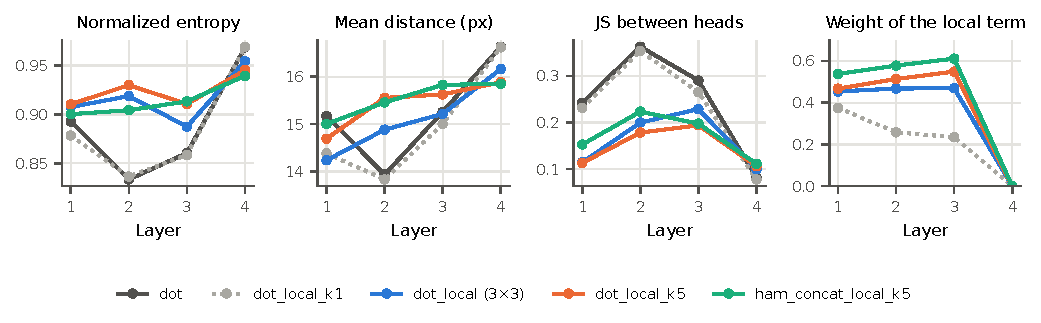
\includegraphics[width=\textwidth]{figuras/mecanismo.pdf}
  \caption{Attention per layer on CIFAR-10 (mean of 16 seeds; 5 for \var{dot\_local\_k1}). From left to right: normalized entropy of the attention rows, mean attention distance, JS divergence between heads and fraction of the output norm contributed by the local term.}
  \label{fig:mecanismo}
\end{figure*}

\subsubsection{Comparison with the Fusion Mechanisms}
\label{sec:res-colapso}
Table~\ref{tab:colapso} explains why the fusions of the first family do not improve on \var{dot}. In score mixing, one of the two branches dominates and the other becomes irrelevant; which one wins depends on the relative scale of the scores:
\begin{itemize}
  \item with $\lambda=0.85$, the applied attention is almost that of \var{dot} (JS of 0.016--0.035) and far from the additive one (0.27--0.39);
  \item with the sum, the free additive, whose scores reach $\pm d$, dominates (JS of 0.005--0.056) and the \var{dot} branch becomes almost uniform (entropy of 0.96--1.00);
  \item when the additive branch is scaled by $1/\sqrt{d}$, it flattens (entropy of 0.94--0.97) and \var{dot} wins (JS of 0.001--0.004).
\end{itemize}
This is the expected consequence of score mixing being a product of distributions (Section~\ref{sec:fusiones}): the sharper branch decides. Standardizing the scores (\var{ham\_zscore}) and mixing outputs instead of scores avoid the collapse: the applied attention differs from both branches and the \var{dot} branch contributes between 60 and 77~\% of the output. But they do not improve accuracy either (Table~\ref{tab:fusiones}). Moreover, when $\lambda$ is learned, its final value depends on the initialization: the same output-mixing model ends with $\lambda_{\text{dot}}$ of 0.65--0.76 if it starts at 0.85, and of 0.23--0.40 if it starts at 0.5, with a 0.79-point difference in accuracy (5 of 5 seeds, $p=0.007$). The problem with these fusions is not only collapse: two similarity functions computed on the same queries and keys do not provide complementary information.

% Translated by scripts/tables_en.py from the Spanish table generated by scripts/ieee_tables.py a partir de los runs; no editar a mano.

\begin{table*}[!t]
\centering
\footnotesize
\caption{Use of the two branches in the CIFAR-10 fusions (mean over seeds 0--4; range over the 4 layers). JS: Jensen--Shannon divergence (base 2) between the attention applied to $v$ and each branch. $H$: normalized entropy of each branch (1 = uniform). Contribution: fraction of the output norm contributed by \texttt{dot}, in output fusions.}
\label{tab:colapso}
\begin{adjustbox}{max width=\linewidth}
\begin{tabular}{lccccc}
\toprule
Variant & JS(fus., dot) & JS(fus., additive) & $H$ dot & $H$ additive & Contrib. dot \\
\midrule
\texttt{ham\_weighted} & 0.016--0.035 & 0.274--0.391 & 0.86--0.97 & 0.57--0.68 & --- \\
\texttt{ham\_weighted\_learn} & 0.058--0.118 & 0.219--0.292 & 0.87--0.97 & 0.59--0.70 & --- \\
\texttt{ham\_sum} & 0.115--0.254 & 0.005--0.056 & 0.96--1.00 & 0.82--0.92 & --- \\
\texttt{ham\_weighted\_scaled} & 0.001--0.004 & 0.044--0.165 & 0.81--0.96 & 0.94--0.97 & --- \\
\texttt{ham\_zscore} & 0.130--0.282 & 0.079--0.186 & 1.00 & 0.90--0.99 & --- \\
\texttt{ham\_weighted\_learn\_out} & 0.022--0.042 & 0.085--0.221 & 0.85--0.97 & 0.71--0.84 & 0.60--0.73 \\
\texttt{ham\_wout} & 0.009--0.045 & 0.086--0.215 & 0.82--0.96 & 0.75--0.84 & 0.60--0.76 \\
\texttt{ham\_gated} & 0.012--0.054 & 0.098--0.230 & 0.83--0.96 & 0.77--0.85 & 0.63--0.77 \\
\texttt{ham\_concat} & --- & --- & 0.85--0.96 & 0.78--0.85 & 0.53--0.60 \\
\bottomrule
\end{tabular}
\end{adjustbox}
\end{table*}


\subsection{Ablations of the Output Terms}
\label{sec:res-ablacion}
Ablations with seeds 0 to 4 (Supplementary Section~\ref{sec:sup-ablacion}, Table~\ref{tab:ablacion} and Fig.~\ref{fig:kernel}) locate the gain of the output terms:
\begin{itemize}
  \item \textbf{It comes from the neighborhood.} With $k=1$ (\var{dot\_local\_k1}), the term keeps the additional value path but does not mix neighboring patches, and the accuracy is that of \var{dot} ($+0.07$ [$-0.52$, $+0.67$]).
  \item \textbf{It saturates at $5\times5$.} A $7\times7$ kernel, which almost covers the $8\times8$ grid, is only $+0.20$ [$-1.19$, $+1.60$] from $5\times5$.
  \item \textbf{It is not a capacity effect.} With 16 paired seeds, \var{dot\_wide\_local\_k5} is $+0.17$ [$-0.59$, $+0.94$] from \var{dot\_local\_k5}.
  \item \textbf{The gate and the residual global context do not help}, either alone or on top of the local term; with 16 seeds, the gate on top of the local term gives $-0.11$ [$-0.50$, $+0.28$].
  \item \textbf{Other ways of combining mechanisms with the local term do not separate from it.} With 16 seeds, splitting the branches across heads gives $+0.19$ [$-0.49$, $+0.87$] over \var{dot\_local\_k5}, and removing pairwise attention altogether (only the \emph{pooling} branch with the local term, without any $N\times N$ matrix) gives $-0.47$ [$-1.24$, $+0.30$], still $+5.17$ over \var{dot}.
\end{itemize}

\subsection{Fulfillment of the Criteria}
\label{sec:res-criterios}
No variant meets all four criteria set in advance (Table~\ref{tab:criterios}). \var{dot\_local\_k5} meets the gain over the capacity control, the sign on another dataset and the cost; the per-branch contribution criterion does not apply because it has a single attention branch, and its local term contributes 47 to 55~\% of the output in layers 1 to 3. \var{ham\_concat\_local\_k5} meets three: the gain over its capacity control (with the 48 seeds, Holm $p=0.031$), the balance between branches and the same sign of that contrast on PlantVillage ($+0.23$ over \var{dot\_wide\_local\_k5}); it fails the cost criterion, at 1.78 times the epoch time of \var{dot}. \var{ham\_concat} meets the branch balance and the sign on PlantVillage ($+0.24$ over \var{dot\_wide}), but does not separate from its capacity control on CIFAR-10 and costs 1.68 times the epoch time of \var{dot}. The score fusions only meet the sign criterion, because they improve on \var{dot} on PlantVillage.

% Translated by scripts/tables_en.py from the Spanish table generated by scripts/ieee_tables.py a partir de los runs; no editar a mano.

\begin{table*}[!t]
\centering
\footnotesize
\caption{Fulfillment of the four criteria set in advance (Section~\ref{sec:analisis}). C1: paired gain on CIFAR-10 over the equal-capacity control (\texttt{dot} for score fusions, which add no parameters) with Holm $<0.05$ over the 8 comparisons and at least 10 seeds. C2: no branch contributes less than 10\,\% of the output norm; for score fusions, which have no separate outputs, the JS divergence between the applied attention and each branch is used (JS $\approx0$: the fusion is that branch); n/a: a single attention branch. C3: the C1 contrast, against the same control, has $\Delta>0$ on another dataset (PV: PlantVillage, batch 128; Food: Food-101; seeds 0--4, paired t-test $p$ in parentheses). C4: epoch time $<1.5$ times that of \texttt{dot}.}
\label{tab:criterios}
\begin{adjustbox}{max width=\linewidth}
\begin{tabular}{>{\raggedright\arraybackslash}p{3.25cm}>{\raggedright\arraybackslash}p{3.5cm}c>{\raggedright\arraybackslash}p{2.85cm}c>{\raggedright\arraybackslash}p{3.0cm}ccc}
\toprule
Variant & C1: gain &  & C2: contribution per branch &  & C3: other datasets &  & C4: cost &  \\
\midrule
\texttt{ham\_weighted} & $-0.38$, Holm 0.367 & no & fusion = \texttt{dot} (JS $\leq$0.035) & no & PV: $+0.08$ (0.534)\newline Food: not evaluated & yes & 1.89$\times$ & no \\
\texttt{ham\_sum} & $-0.55$, Holm 0.077 & no & fusion = \texttt{additive\_free} (JS $\leq$0.056) & no & PV: $+0.64$ (0.007)\newline Food: not evaluated & yes & 1.95$\times$ & no \\
\texttt{ham\_concat} & $+0.48$, Holm 0.017\newline vs.\ \texttt{dot\_wide}: $+0.15$, Holm 0.491 ($n=16$) & no & minor branch: 0.40 & yes & PV: $+0.24$ (0.046)\newline Food: control not evaluated & yes & 1.68$\times$ & no \\
\texttt{dot\_local\_k5} & $+5.64$, Holm $<0.001$\newline vs.\ \texttt{dot\_wide}: $+5.31$, Holm $<0.001$ ($n=16$) & yes & single attention branch; local term 0.47--0.55 (layers 1--3) & n/a & PV: $+0.56$ (0.024)\newline Food: not evaluated & yes & 1.08$\times$ & yes \\
\texttt{ham\_concat\_local\_k5} & $+6.31$, Holm $<0.001$\newline vs.\ \texttt{dot\_wide\_local\_k5}: $+0.61$, Holm 0.031 ($n=48$) & yes & minor branch: 0.37 & yes & PV: $+0.23$ (0.089)\newline Food: not evaluated & yes & 1.78$\times$ & no \\
\bottomrule
\end{tabular}
\end{adjustbox}
\end{table*}

